\section{High level components and their interaction}
\label{sec:high-level}

The main high level components of the system are the following:
\begin{itemize}
	\item Application server
	\item Web server
	\item Mobile application
	\item Data base
	\item Server side plug-ins:
		\begin{itemize}
		\item ride sharing
		\item ride rieservation
		\end{itemize}
	\item User's browser
\end{itemize}

The main components are structured into four layers presented in figure \ref{fig:layers}, which are the following:
\begin {enumerate}
	\item Data base
	\item Application server
	\item Web server
	\item Client
\end{enumerate}

\begin{figure}[h]
\centering
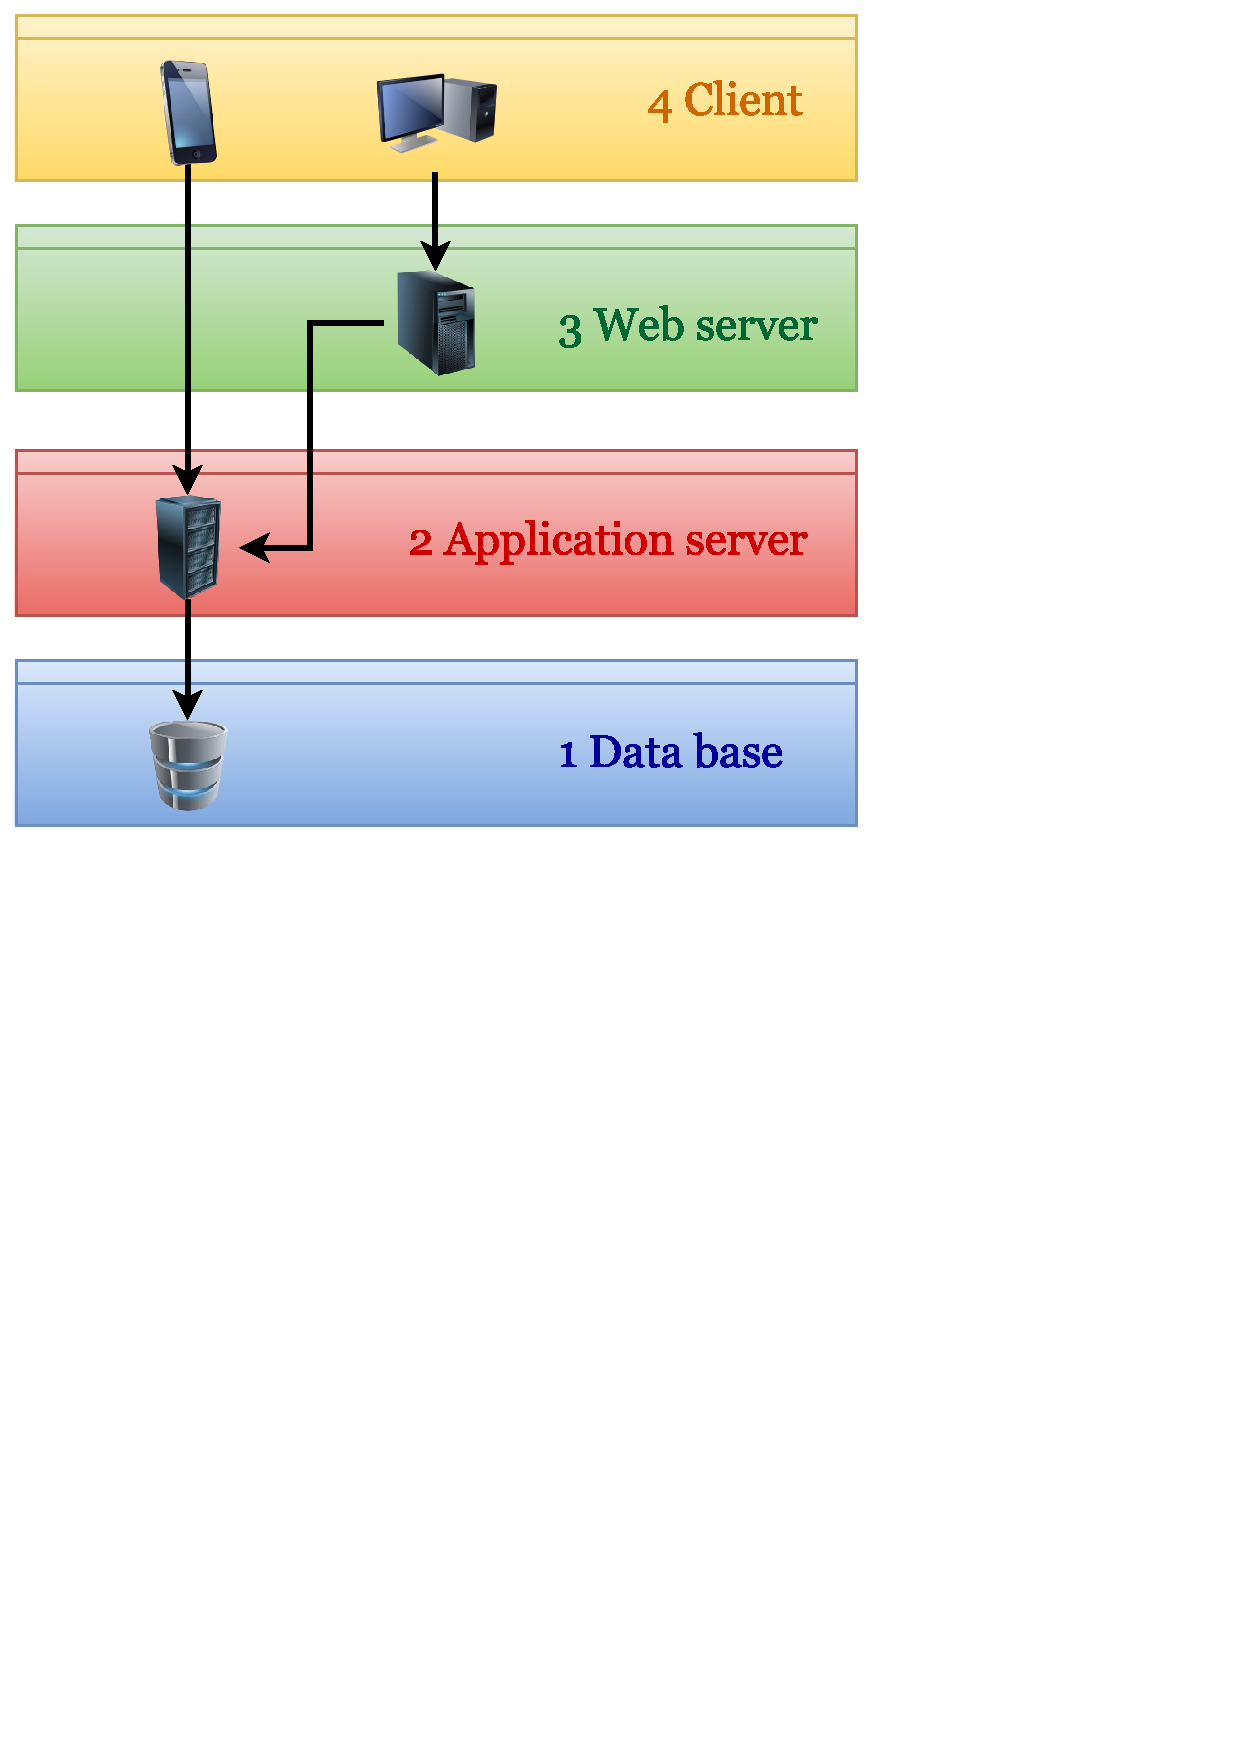
\includegraphics[width=\textwidth]{diagrams/layers.pdf}
\caption{Layers of the system.}
\label{fig:layers}
\end{figure}

The interactions between the main components are shown in the figure \ref{fig:high_level_components} and are asynchronous.

\begin{figure}[h]
\centering
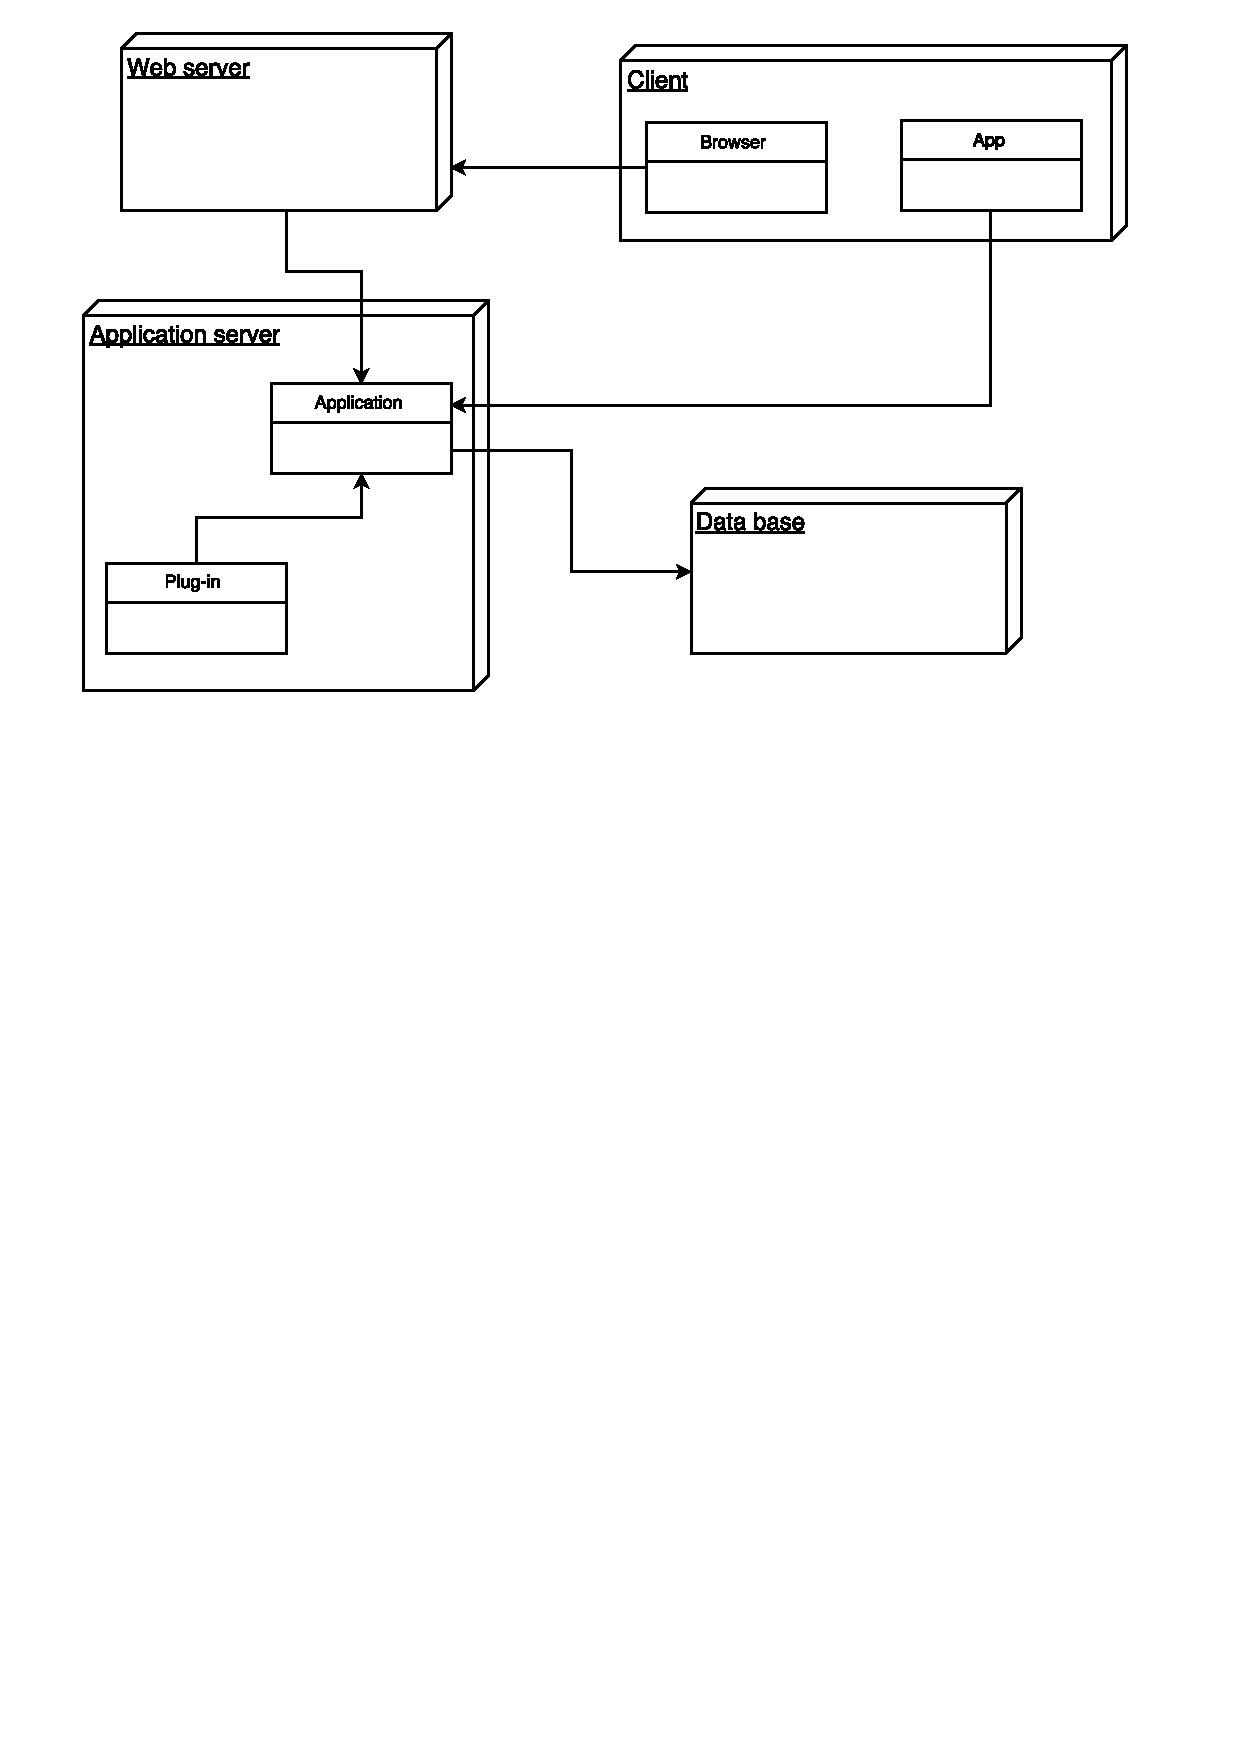
\includegraphics[width=\textwidth]{diagrams/high_level_components.pdf}
\caption{High level components of the system.}
\label{fig:high_level_components}
\end{figure}